\chapter{Methodology}
\label{cha:methodology}

With the scope of the work now defined, the manner in which the required results will be obtained can now be detailed. The necessary additions as defined in Section \ref*{sec:intro_scope}, Scope, may will be implemented in the form of two independent assemblies in order to meet the requirements of the work. These two assemblies will be refereed to as the Processor Module and the Magnetic Separation Station. The former will be the site of the chemical reactions as described in Section \ref{subsec:intro_extraction}, The Extraction Process, and will be the hardware element that forms the SBS block on the Gene-Plex Extractor deck. Therefore, given it will house the full set of reactions, it will also encompass the software and hardware requirements of the liquid temperature control (including the associated controller), along with the magnetic separation required in tube number 4 of the cassette. The Magnetic Separation Station will be the location of disposal of the supernatant and therefore shall include the magnetic hardware required to physically manipulate the magnetic silica beads in order to retain them in the pipette tip while the waste is expelled. Given the biological nature of the liquid waste involved, this station will also include provisions for hygienically disposing of and storing this waste.

\section{Processor Module}

\subsection{Hardware}

%NOTE : need to atleast mention use of autodesk CFD and rough method

The hardware component of the Processor Module design is concerned with ensuring the module accepts the required cassette tubes, fits within the stipulated SBS space and provides a stable platform for the required temperature control using the knowledge gained in Section \ref{lit_controlability}, Controllability. The work in this sections will also include the selection of an appropriate heat pumping device. In order to ensure the requirements of the hardware elements are met, the design process is applied as follows:
\begin{enumerate}
	\item Generation of concepts related to thermally isolating the heated and non-heated regions of the block. This includes a focus on the manufacturability of the resulting components.
	\item Investigation into and selection of an appropriate heating method.
	\item Full CAD design of hardware including provisions to accommodate the required tubes.
	\item Utilization of 3D printing to test the fit of the cassette tubes in the block design.
	\item CFD simulation using Autodesk CFD Motion to verify the performance of the selected heating element and the thermal stability of the final design. 
\end{enumerate} 

\subsection{Temperature Controller}

This work will result in the finalisation of a software temperature controller capable meeting the liquid heating requirements of the chemical reaction as detailed in Section \ref{subsec:intro_extraction}, The Extraction Process.

In order to enable controller design to be commenced, the first step will be to assemble the completed Processor Module. Due to the complex dynamics of the heat transfer between the heating device and the liquid, a mathematical modelling method is not used. Instead, the system will be identified via the step input response plant identification method. To obtain the required response data, sensors will be placed strategically on the Processor Module to monitor and record key temperatures:
\begin{itemize}
	\item The temperature at the centre of the block will be taken as this sensor data will be utilized as feedback for the controller to be implemented. This follows the recommendations given in Section \ref{cha:literaturereview} by Vilchiz et. al.
	\item The temperature of the heatsink will be plotted to monitor the temperature differential created across the module.
	\item The temperature of the heated region of the module will be taken on its outer surface to determine the success of the design in creating a component that responds to temperature control in responsive and stable manner.
	\item The temperature of the liquid within the cassette tubes will be measured as the final output of the system. The ability of the controller to drive this temperature to the desired set point will determine the success of the design.
\end{itemize}

To utilize this data for experimental plant identification, an Arduino will be used as an interface between the sensor electronics and MATLAB. This will enable the real-time monitoring and plotting of the data along with storage and subsequent analysis through the Arduino's Analogue input ports.\\

With the hardware now setup, the Processor Module will then be excited by a step input. The input will be provided by the same controlling electronics used in the final Processor Module. As was detailed in Section \ref{sec:intro_scope}, Scope, the companies MTX Cycler electronics driver board will be utilized. The software controlling this board will therefore be modified to provide a constant step input to the Processor Module. The step input will be applied and the response data logged until a steady state has been achieved.\\

This data will have been logged in the MATLAB workspace in real-time, during the experiment. Prior to analysis however, the data will be pre-processed to remove any unnecessary features. For example, the data will be seroed so that the response data begins at time $t = 0$ and so that the response begins at $0\degree$C. This will remove any effects of the varying room temperature at which the experiment may occur and ease the fitting of curves to the collected data.\\

To complete the plant analysis process using the pre-processed data, the MATLAB PID Tuner tool will be used. This tool provides a GUI for specifying a set of response data, the step input provided. This information is then used to interactively fit an appropriate function to the plants response data. The tool offers a number of plant structures to allow the correct plant to be identified. These range from a simple "One Pole" plant to a discrete time system.\\

As a result of this process, the transfer function which represents the plant of the Processor Module will be known. This plant will be in the continuous time domain and is represented by:

$$G_p(S)$$

Before utilizing the identified plant for controller design, it will be verified via simulation in Simulink. The validation will be conducted by providing the plant an identical step input as was done experimentally and verifying that the responses match. The Simulink layout used to conduct this simulated verification is shown below in Figure \ref{fig:openloopplant}.\\

\begin{figure}[!htb]
	\centering
	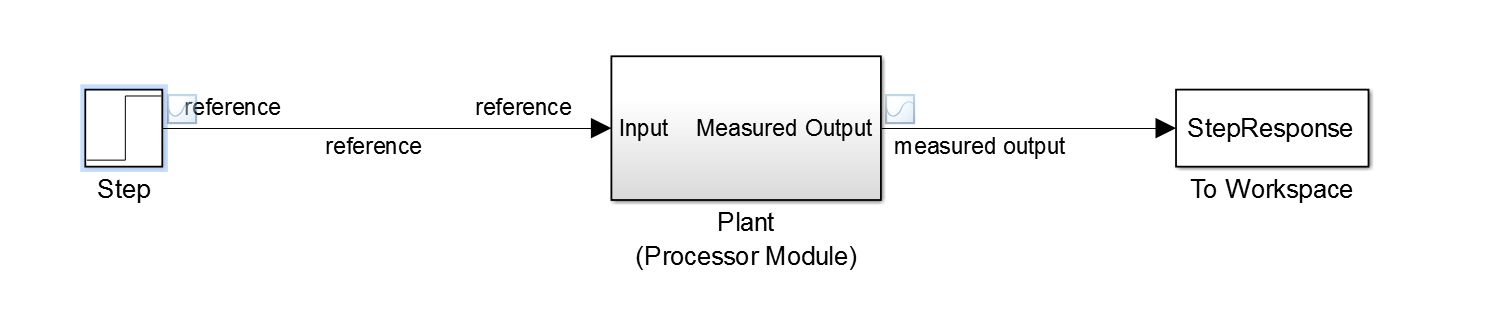
\includegraphics[width = \textwidth]{openloopplant.png}
	\caption[Open loop plant valiation Simulink Model.]{The Simulink model layout used to validate via simulation the identified plant for the Processor Module.}
	\label{fig:openloopplant}
\end{figure}ˆ 
\FloatBarrier

With the transfer function representing the Processor Module now known, the process of controller design may be commenced. The method chosen for this design process is the Direct Analytical Method (also known as Ragazzini's Method), in the discrete time domain. As was noted in Chapter \ref{cha:literaturereview}, Literature Review, the most common method of control for thermal cycling devices in similar applications is PID control. This method has not been selected however due the benefits of competing controller design in the z-domain with discrete time. By completing the design entirely in the z-domain, there is no need to convert the resulting controller from the s domain, allowing the controller to be directly implemented.\\

The direct analytical method uses the principle that if the output that is required along with the input applied is known the intermediate transfer function may be determined. This is represented by Equation \ref{eq_direct}, where $C(z)$ is the required output, $U(z)$ is the applied input and $F(z)$ is the intermediate transfer function.

\begin{equation}
\label{eq_direct}
C(z) = F(z)U(z)
\end{equation}

The method of feedback used for the controller is a unity feedback signal. Data provided by the utilized sensor will be processed to give a feedback signal with unity gain, to ensure any features of the raw signal are removed. For the unity feedback system picture in Figure \ref{fig:unityfeedback}, $F(z)$ is given as \cite{UNSW}:

\begin{equation}
F(z) = \frac{G_c(z)G_p(z)}{1+G_c(z)G_p(z)}
\end{equation}

\begin{figure}[!htb]
	\centering
	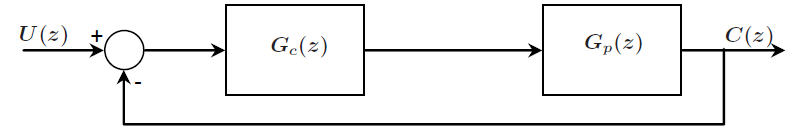
\includegraphics[width = \textwidth]{unityfeedback.png}
	\caption[Unity feedback system.]{The block diagram for a unity feedback system. \cite{UNSW}}
	\label{fig:unityfeedback}
\end{figure}ˆ 
\FloatBarrier

Due to the plant identification completed earlier, the continuous time form of the system plant is known. Using MATLAB, this may be converted to a discrete time transfer function, with the appropriate sampling time selected. Therefore, $G_p(z)$ is known.\\

Rearranging for the controller of interest, $G_c(z)$ gives:
\begin{equation}
\label{eq_controller}
G_c(z) = \frac{F(z)}{G_p(z)[1-F(z)]}
\end{equation}

By equation \ref{eq_controller}, the direct method requires only that $F(z)$ be determined to realise the controller. To complete the formation of $F(z)$ and hence $G_c(z)$, the method below will be utilized. This method, as detailed by J. Katupitiya \cite{UNSW}, provides a number of steps to ensure the resulting controller performs as required.\\

\subsubsection{Controller Performance}

To define the response time of the controller, the pole locations are set. To do so, the desired time constant of the system, $\tau$ is set and the s domain pole is found by:

\begin{equation}
s = -\frac{1}{\tau}
\end{equation}

This s domain pole is then transferred to the z domain via:

\begin{equation}
z = e^{sT}
\end{equation}

Where T is the sample time of the controller. The resulting pole is then placed as a pole of $F(z)$.\\

It is also important to control the steady state error of the controller. To do this, the DC gain of the system is set to 1, resulting in the output equalling the input at steady state. By setting the following, this can be achieved:

\begin{equation}
F(z)|_{z=1} = F(1) = 1
\end{equation}

\subsubsection{Pole Zero Cancellation}

It must be ensured that a pole or zero cancellation does not occur in the unstable region of the Z-Plane, in order to ensure that this cancelled pole does not become a component of the formed characteristic equation. If a controller component cancels an unstable plant pole or zero in this scenario, it will influence the system so that it becomes unstable. These constraints will be dealt with via two stability constraints:\\

\textbf{Stability Constraint 1}\\
Stability constraint 1 addresses the instability that may occur if a pole of the plant $G_p(z)$ is cancelled by a zero of $G_c(z)$. Firstly, all poles of $G_c(z)$ are tested for instability, where any pole $z = p_0$ is unstable if :

\begin{equation}
\label{eq_unstablepole}
|p_0| > 1
\end{equation}

If any pole is found to satisfy Equation \ref{eq_unstablepole}, it is unstable and must be added as a zero of $[1 - F(z)]$. This addition removed the unstable pole and ensures the controller is not able to create the unstable cancellation.\\

\textbf{Stability Constraint 2}

Stability Constraint 2 deals with the case that an unstable zero exists in the plant transfer function. Therefore, it prevents a pole of the controller from cancelling this zero in the unstable region. A zero of the controller $G_c(z)$, $(z = z_0$ may be tested for instability by checking if it satisfies Equation \ref{eq_unstablezero}:

\begin{equation}
\label{eq_unstablezero}
|z_0| > 1
\end{equation}

Any zero satisfying this equation can be identified as unstable and dealt with by including it as a zero of $F(z)$.\\

\textbf{Causality Constraint}

The causality constraint ensures that the designed controller is either proper or strictly proper. That is, that it only uses current or past terms in the calculation of controller effort and no futuristic terms. This is achieved by ensuring the pole-zero deficiency of the plant (i.e. its delay) is either that same as or less than that of $F(z)$. The pole-zero deficiency of he plant is the order of the denominator minus the order of the numerator, denoted as:

\begin{equation}
\label{eq_plantdef}
D[ G_p(z) ] = n
\end{equation}

The pole zero deficiency of $F(z)$ is given as:

\begin{equation}
\label{eq_fdef}
D[ F(z) ] = m
\end{equation}

If $m = n$, the controller is strictly proper. If $m > n$, the controller is proper. However, if $m < n$, then the controller is improper (will require futuristic terms) and the causality constraint is not satisfied. In this situation, the order of the denominator of $F(z)$ must be increased until the controller is at least strictly proper.\\

\textbf{Controller Difference Function}

Using the $F(z)$ found using the previous steps, the controller transfer function, $G_c(z)$ can then be calculated. This transfer function is converted into a function of the variable $Z^{-1}$, which is commonly known as the Digital Signal Processing (DSP) format. This allows the transfer function to be directly written as a difference function involving multiple error and controller effort terms with varying time delays. This difference function is the realised discrete controller.\\

\textbf{Simulated Validation}

In order to validate the design of the controller prior to implementation, the design will be simulated via Simulink to validate its response to the desired reference input. The block diagram shown in Figure \ref{fig:controllervalidation} will be used to conduct the validation and record the resulting data. The response recorded will be assessed against the controller requirements.

\begin{figure}[!htb]
	\centering
	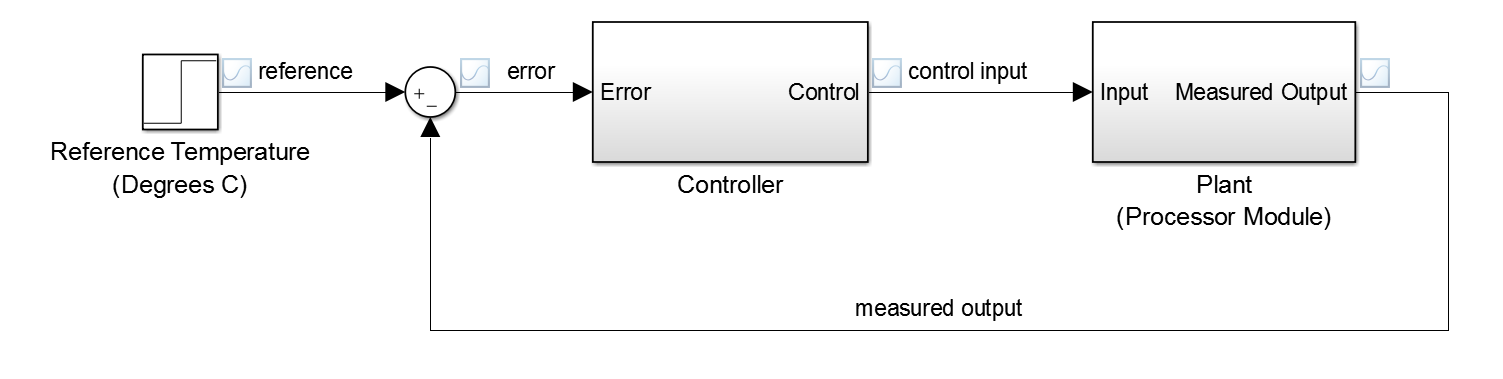
\includegraphics[width = \textwidth]{controllervalidation.png}
	\caption[Controller valiation Simulink Model.]{The Simulink model layout used to validate via simulation the designed controller for the Processor Module.}
	\label{fig:controllervalidation}
\end{figure}ˆ 
\FloatBarrier

Following the successful validation of the temperature controller, it will be implemented via software currently driving the MTX cycler, along with any required modifications.

%UP TO HERE

\subsubsection{Experimental Verification}

In order to verify the performance of the resulting controller, the following experimental verification will be conducted. The experiment will determine the ability of the controller to meet the steady state error, disturbance rejection, response time, overshoot and stability requirements when controlling temperature in the module. The method is as follows:

\begin{enumerate}
	\item Assemble 4 complete Processor Modules
	\item Using an Arduino as an interface and MATLAB as the data logger and analyser, measure the temperature in the tubes shown in Figure \ref{fig:measuredtubes} for the duration of the experiment.This distribution will allow the performance at the extremes of the device to be determined.
	\begin{figure}[!htb]
		\centering
		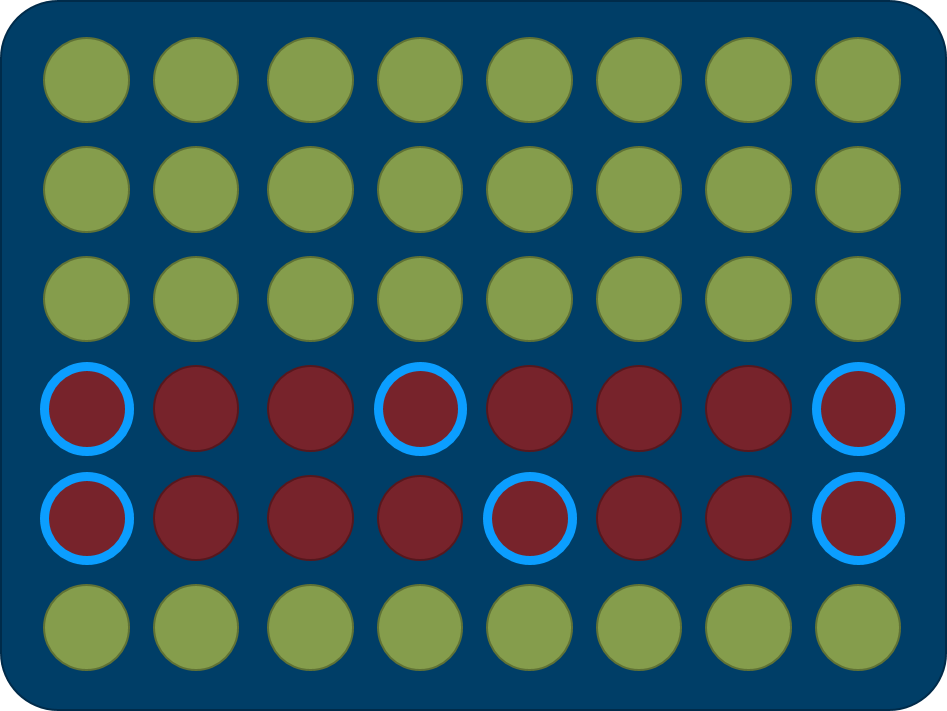
\includegraphics[width = \textwidth]{measuredtubes.png}
		\caption[Temperature Measured Tubes.]{Tube locations to be measured during temperature control verifications experiment. Non-Heated tubes are coloured green, heated tubes are coloured red, measured tubes are outlined in blue.}
		\label{fig:measuredtubes}
	\end{figure}ˆ 
	\FloatBarrier
	\item Begin data logging and live plotting.
	\item Set the reference input to the controller to 60$\degree$C.
	\item Collect data for a total of 30 minutes to capture the long term steady state performance of the module (to allow any slow heat transfers to be observed) along with the transient response.
	\item Repeat the experiment for all four assembled modules. This allows for the controllers ability to reject disturbances caused by the differing of the plant properties to be determined as is caused by the slight differences in assembly.
	\item Repeat experiment in differing environmental conditions. The experiment should  be conducted in rooms at temperatures of 18$\degree$C, 22$\degree$C and 26$\degree$C. This allows for the disturbance rejection of the controller to be assessed where the disturbance is due to altered environmental conditions.
	\item Use the collected data to assess the consistency of the heating profile and the temperature stabilisation across the tubes of the module. These results will be used to make conclusions regarding the designed controller along with the thermal characteristics of the hardware. It should be noted that the worst case response will be used to draw conclusions regarding performance to ensure all samples fall within the requirements.
\end{enumerate}

\subsection{Magnetic Separation}

As the final stage of the extraction process is the removal of the clean sample from the waste beads, the success of extraction depends on the complete and reliable separation in tube number 4. To ensure this is achieved, the following design process and experimental verification will be conducted:
\begin{enumerate}
	\item An investigation will be conducted into the various possible methods of magnetic separation in this application, taking into account the recommendations to use ND-Fe-B magnet compositions as found in the reviewed literature.
	\item 3D Printed test jigs will be created to test the effectiveness of the most suitable configurations via manual inspection.
	\item With a preferred design selected, the a test module will be 3D printed including the magnetic arrangement. This test module will be assembled on the robot deck and verified experimentaly via the method described below.
\end{enumerate}

\subsubsection{Experimental Verification}

To allow a confident conclusion to be made regarding the effectiveness of the magnetic separation within the Processor Module to be made, the following experiment will be conducted. This experiment will replicate the setup used by the robot and its processes to ensure the result is representative of the true scenario.

\begin{enumerate}
	\item Place test module with magnetic separation on Gene-Plex Extractor deck within one of the SBS spaces.
	\item Place a 5mL tube on the robot deck to collect the experiment output.
	\item Place a full set of 8 cassettes in the test module with 100$\mu$L of filtered water and 10$\mu$L of magnetic beads in tube 3. The water will simulate the elution buffer. Both volumes are equal to that used in the final process.
	\item Instruct the robot to aspirate the mixture in tube 3 and expel it into tube 4, the location of the magnetic separation.
	\item Wait for 5 seconds for separation to take place. It should be noted that this waiting period is a design variable and may be adjusted and this experiment repeated to determine the optimal wait time.
	\item Aspirate the separated liquid at a distance of 1mm from the tube bottom. This distance once again may be adjusted, however is a sound starting point for experimentation.
	\item Expel the liquid from the tip into the 5mL tube on the deck.
	\item Repeat this separation procedure for all 8 cassettes.
	\item Refill all cassettes with equal volumes of water and beads, as was defined in step 3.
	\item Repeat the separation for a total of 3 modules to equal the total volume of liquid which will be processed by the Gene-Plex Extractor during the processing of all 24 samples.
	\item Place the 5mL tube with extracted contents adjacent to a large ND-Fe-B magnet to draw any beads to the tube wall. Examine the tube contents for any sign of magnetic beads. The presence of a bead within the tube indicated a failed separation within tube 4. Such a result may lead to severe complications in step 2 (amplification), such as the failed diagnosis of a patient. Therefore, for a successful verification, it is required that no beads are present.
\end{enumerate}

\section{Magnetic Separation Station}

The magnetic separation station is a standalone module on the robot deck which will fulfil two requirements of the extraction process. Firstly, the station will provide the means of separating the waste liquid from the magnetic beads and captured DNA/RNA, as necessary after step 2 (refer to Section \ref{subsec:intro_extraction}) of the extraction process. Following the successful separation of the supernatant, the separation station will provide a means of hygienically disposing of the associated biological waste. The work will be completed via the the methodology described below.

\subsection{Magnetic Separation}

This stage of the extraction process carries a high level of significance in relation to the final result. Poor magnetic separation may effect the reliability of the diagnosis due to a reduction in the sensitivity of the step 2 amplification, or failure of step 3 analysis due to the presence of inhibitors. The former may be caused by a lack of concentration of the target DNA or RNA in the extracted clean sample. Failed magnetic separation could cause this by not properly capturing the magnetic beads and bound target, allowing them to be expelled into waste. This loss of target will lower the sensitivity of the amplifications stage and hence may lower the accuracy of diagnosis. The second scenario of inhibitors may occur if some of the waste liquid remains after washing, contaminating the sample and lowering the effectiveness of the amplification and analysis steps. Therefore, the method used for the design of the magnetic separation capabilities of the Magnetic Separation Station is aimed at ensuring a strong and reliable separation.

\begin{enumerate}
	\item An investigation will be carried out to determine the most suitable magnetic arrangement for providing reliable separation. Similar to the treatment of the magnetic separation capabilities within the Processor Module, the investigation will focus on those employing the ND-Fe-B composition.
	\item The selected configuration will then be implemented as a design concept and a CAD model generated. This detailed design will also account for a number of secondary requirements. These include maintaining a minimum distance between the pipette tip and the Separation Station at all points to remove the possibility of cross contamination occurring through liquid transfer.
	\item The detailed design will then be prototyped using 3D printing to allow experimental verification.
	\item The prototype Separation Station will then be assembled on the Gene-Plex Extractor deck along with the necessary tubes to perform magnetic separation via the experimental procedure detailed below.
\end{enumerate}

\subsubsection{Experimental Verification}

In order to verify the required performance is achieved by the designed Magnetic Separation Station, the following experiment will be performed.

\begin{enumerate}
	\item The prototyped Magnetic Separation Station will be fully assembled and positioned on the deck of the Gene-Plex Extractor.
	\item 3 cassettes and therefore 24 tubes will be positoned on the deck with 640$\mu$L of water and 10$\mu$L of magnetic silica beads in each. These volumes are equal to those used in the extraction process and this will be repeated 24 times, once for each of the 24 samples. Therefore, this setup matches the volumes to be processed by the implemented extractor.
	\item The robot will then be setup to aspirate the liquid mixture from one of the tubes.
	\item The pipette will then be positioned within the magnetic separation station and lowered to full depth. 
	%NOTE THAT A DIAGRAM OF THIS WOULD BE GOOD to show positions
	\item The pipette tip will then be raised and lowered with the full liquid height passing along the magnetic arrangment a total of 2 times.
	%DETERMINE THESE DISTANCES AND PUT IN DIAGRAM
	\item With the beads now separated from the liquid and captured on the pipette wall, the water will be ejected into the waste disposal system. For this experiment, the waste disposal will be replaced by a small glass container that may be used to collect and analyse the ejected liquid.
	\item This procedure will then be repeated for all 24 ``samples".
	\item The contents of the waste container will then be subjected to a magnetic field to collect any beads which were not correctly separated by the process. The presence of any bead within the waste liquid indicated a failed separation.
	%ADD PERCENTAGE TOLERANCES OR VOLUMES 
\end{enumerate}

\subsection{Waste Disposal}

The work on this component of the Magnetic Separation Station is concerned with ensuring the product meets key standards and requirements in order to dispose of the biological waste in a hygienic manner. The disposal of the waste generated by the process is a key factor in ensuring a successful sample extraction. Any failure to safely dispose of this waste may introduce the risk of a cross contamination occurring between two independent samples and therefore a failure to correctly diagnose the patient.\\

To ensure the waste disposal system negates these risks, the process used will focus on researching the related standards initially in order to determine the best practices which must, by regulation, be adhered to. This research will be supplemented by end user feedback. To gain this, a group of key product users will be consulted on preferred methods of waste disposal and hygiene to guide the design process. Using the results of this investigation, the design process will be used to form a final design which takes into account the gathered information and requirements and therefore produce a functional and hygienic waste disposal system.